\section{Pr�sentation des fen�tres}

\subsection{IHM client}

L'IHM Client va permettre de consulter les informations sur le Client.
Elle est appel�e � partir de recherche sur un client sp�cifique. O� � partir d'un lien vers un contact.


\begin{center}
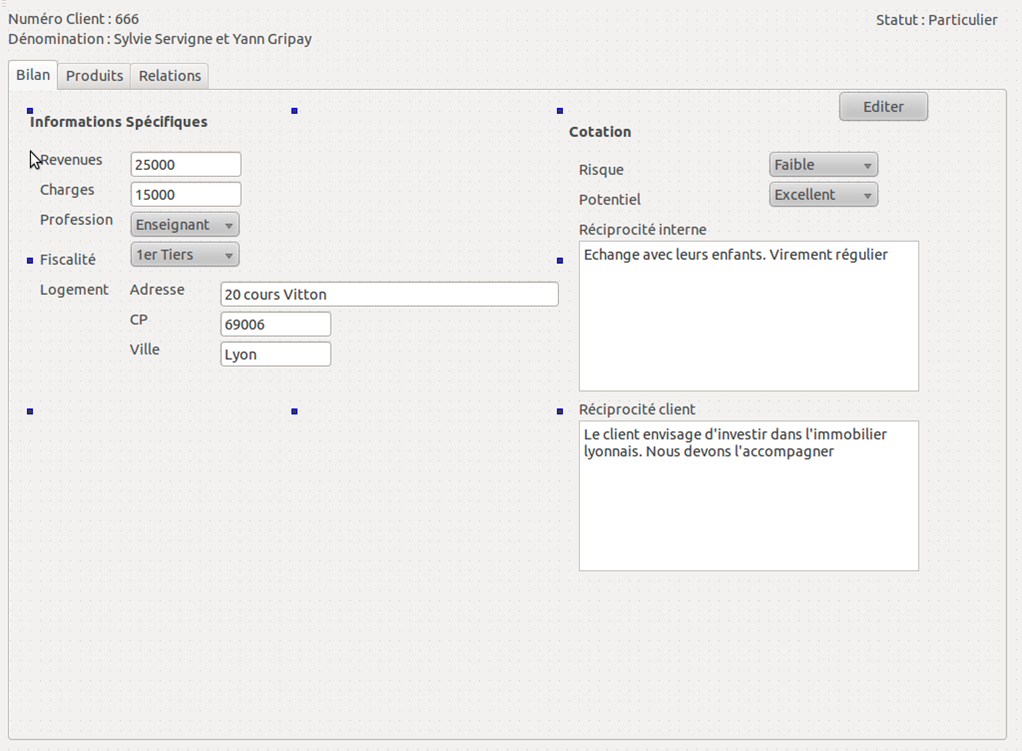
\includegraphics[width=10cm]{\PIXPATH/client1}
\end{center}
\begin{center}
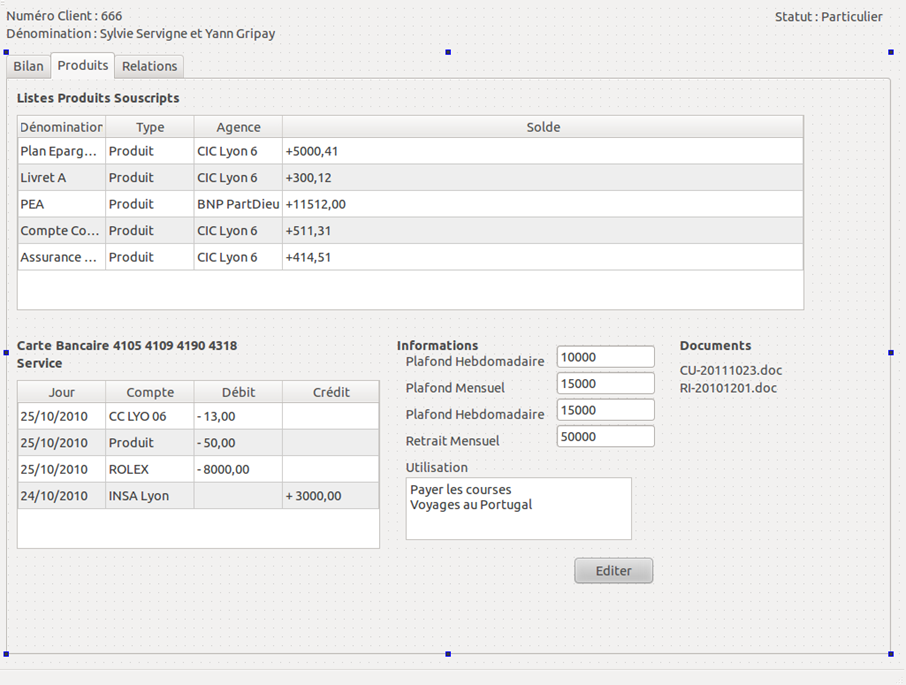
\includegraphics[width=10cm]{\PIXPATH/client2}
\end{center}
\begin{center}
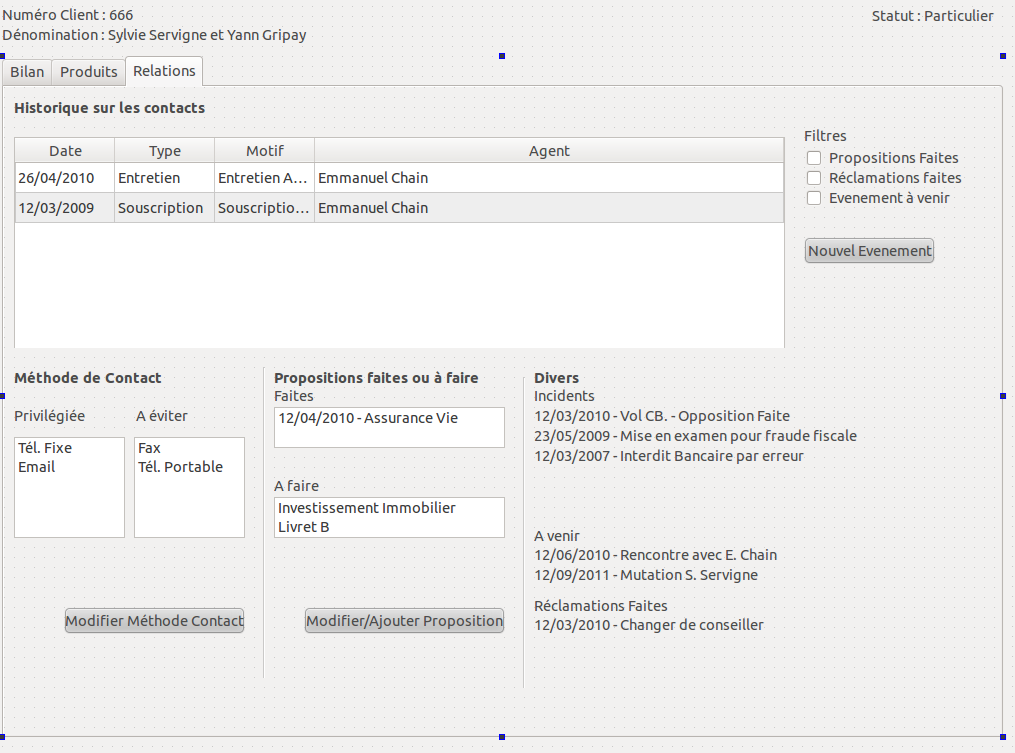
\includegraphics[width=10cm]{\PIXPATH/client3}
\end{center}
%% TODO : remplir

\subsection{IHM Agenda}

L'IHM Agenda permet � un agent de consulter son agenda, mais �galement
celui des autres. En plus de la consultation, il est �galement possible
de g�rer (cr�er, annuler, d�placer, r�affecter) les rendez-vous des
agents de l'agence.

Deux vues sont possibles: une vue par semaine, pour un seul agent; ou
une vue par jour, affichant tous les agents.

Le chef d'agence peut acc�der � un mode �planification� qui lui permet
d'affecter des t�ches � ses agents. Ce mode est disponible pour les
deux types de vues.
\begin{center}
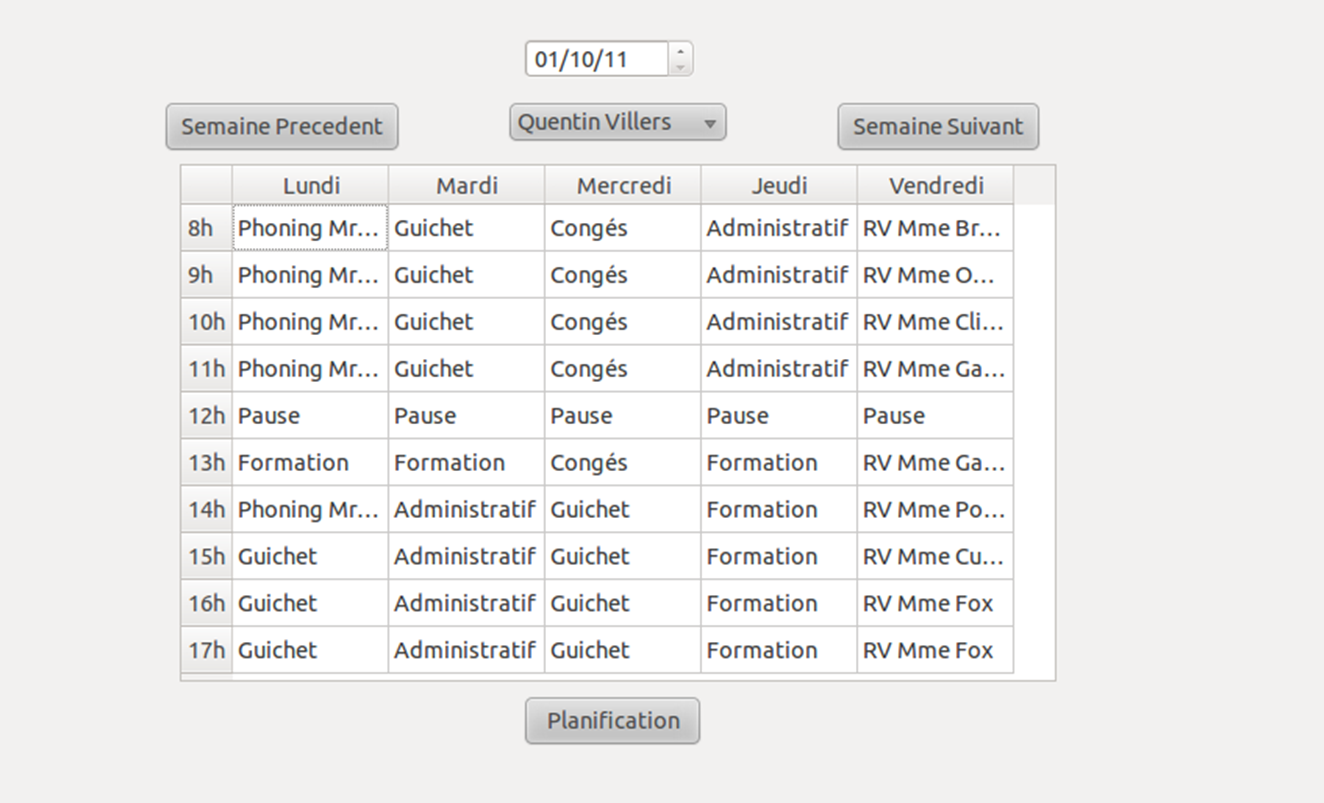
\includegraphics[width=10cm]{\PIXPATH/agenda1}
\end{center}

\begin{center}
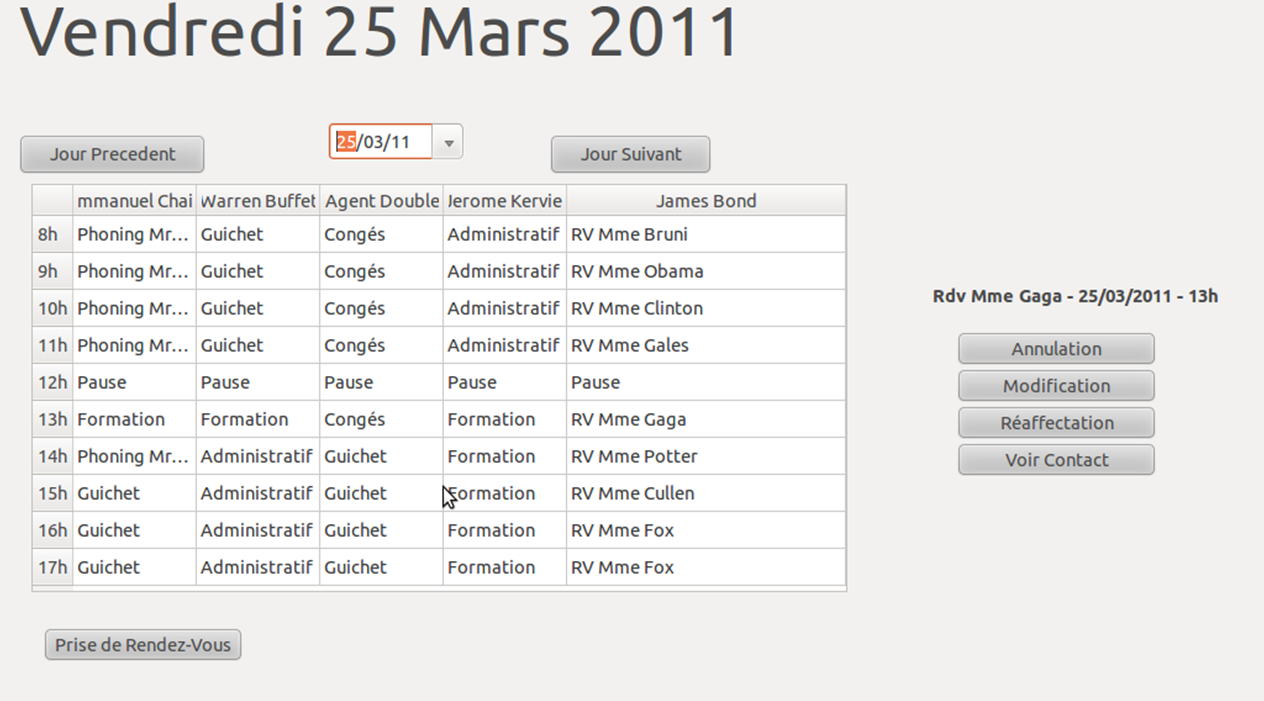
\includegraphics[width=10cm]{\PIXPATH/agenda2}
\end{center}

\subsection{IHM Contact}

L'IHM Contact va permettre � l'agent de pr�parer un compte-rendu de pr�paration
d'entretien et r�diger le RAC.

\begin{center}
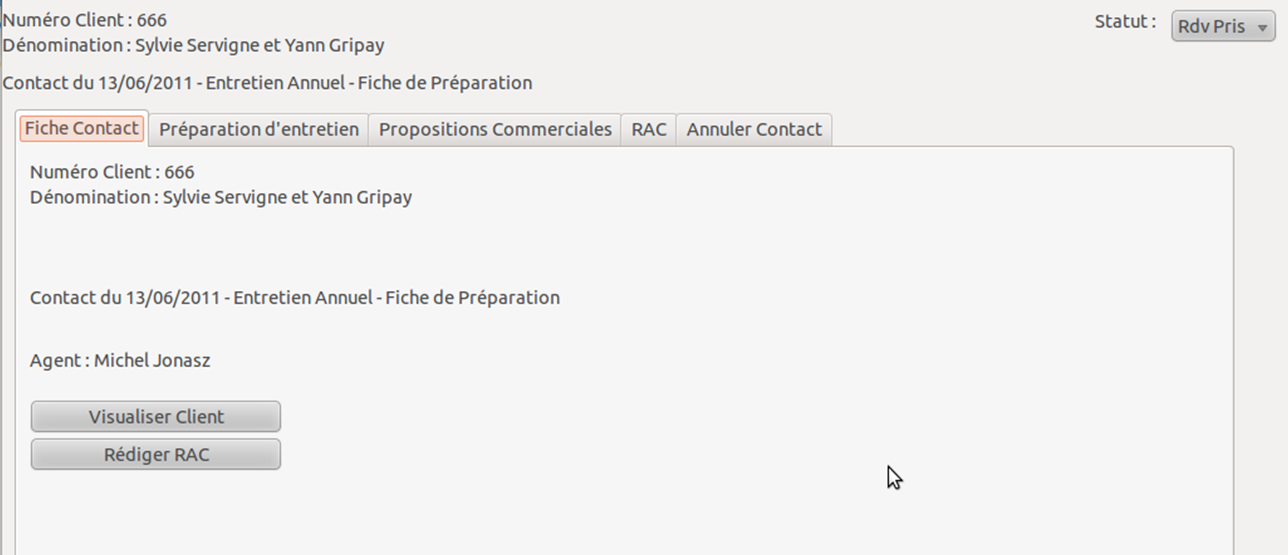
\includegraphics[width=10cm]{\PIXPATH/contact1}
\end{center}
\begin{center}
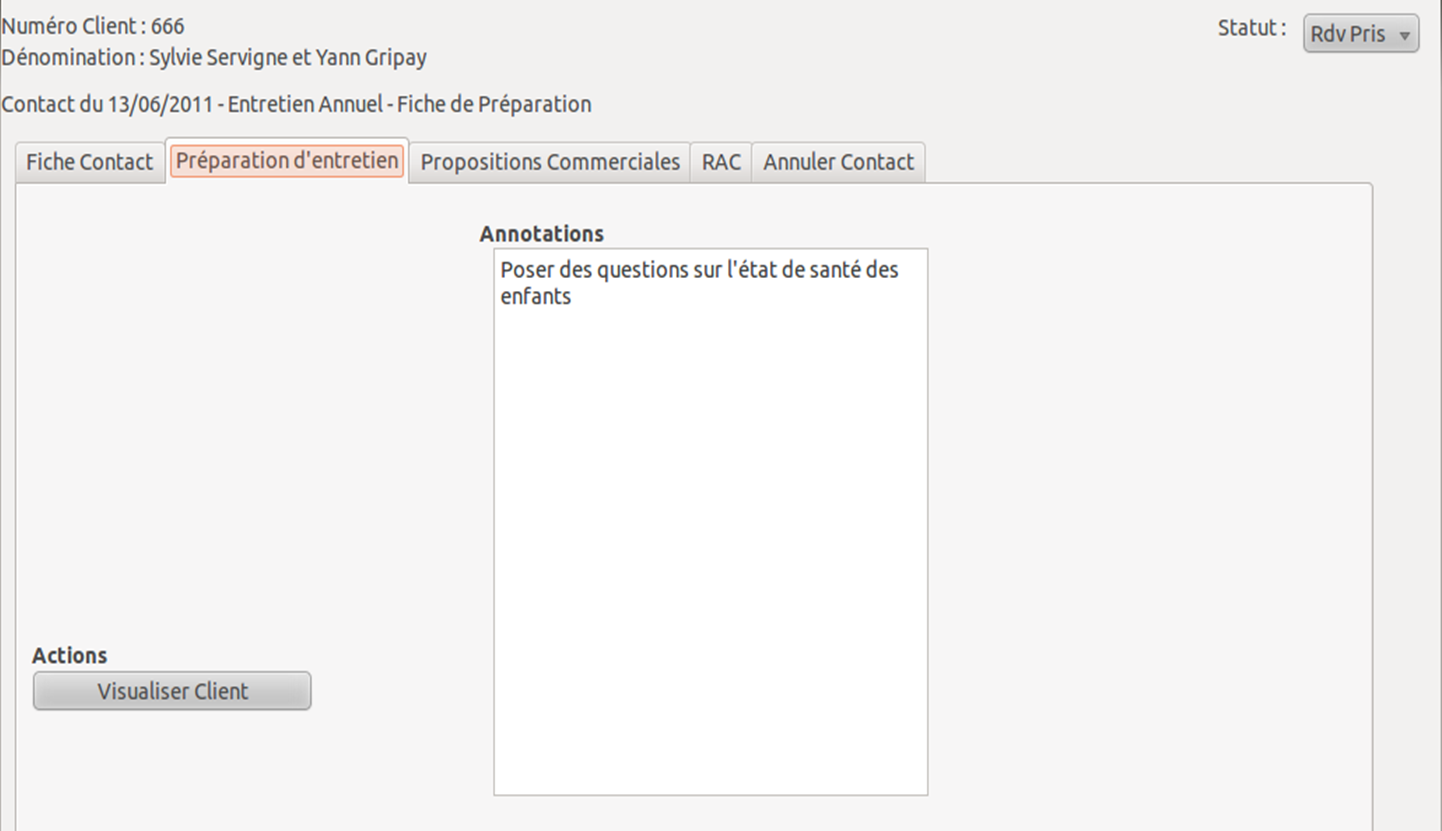
\includegraphics[width=10cm]{\PIXPATH/contact2}
\end{center}
\begin{center}
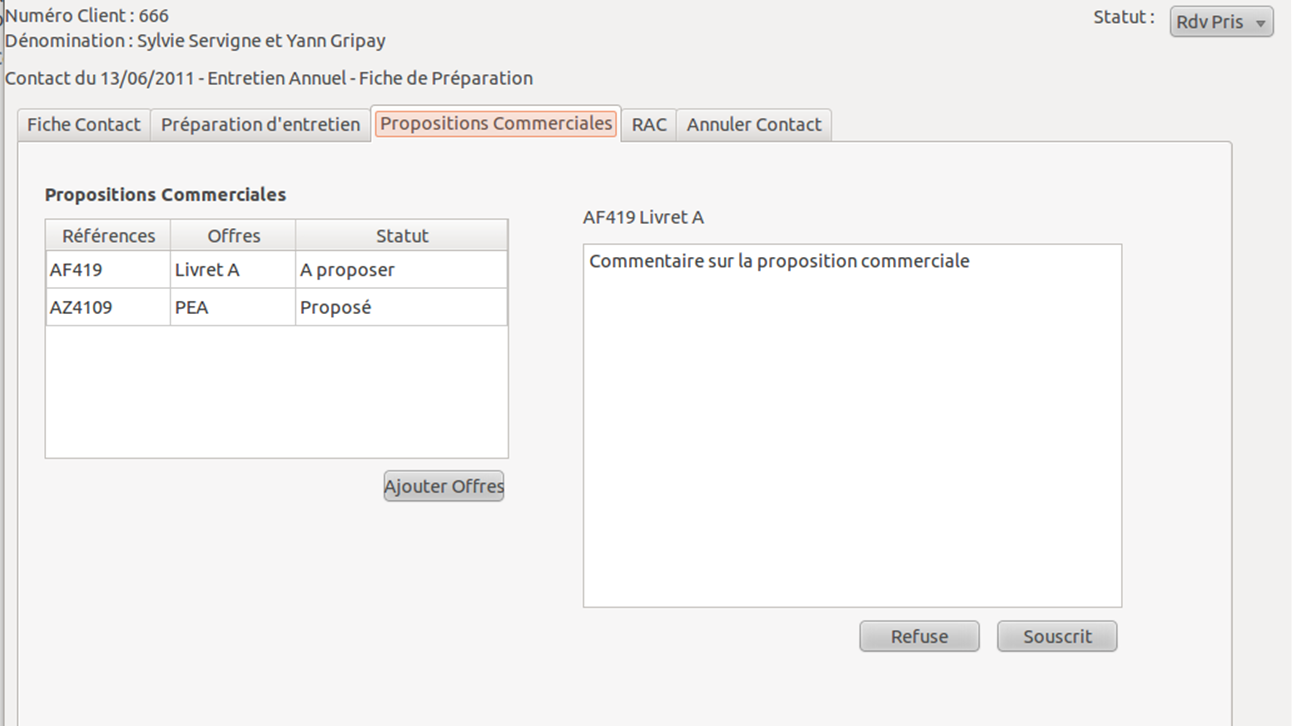
\includegraphics[width=10cm]{\PIXPATH/contact3}
\end{center}
\begin{center}
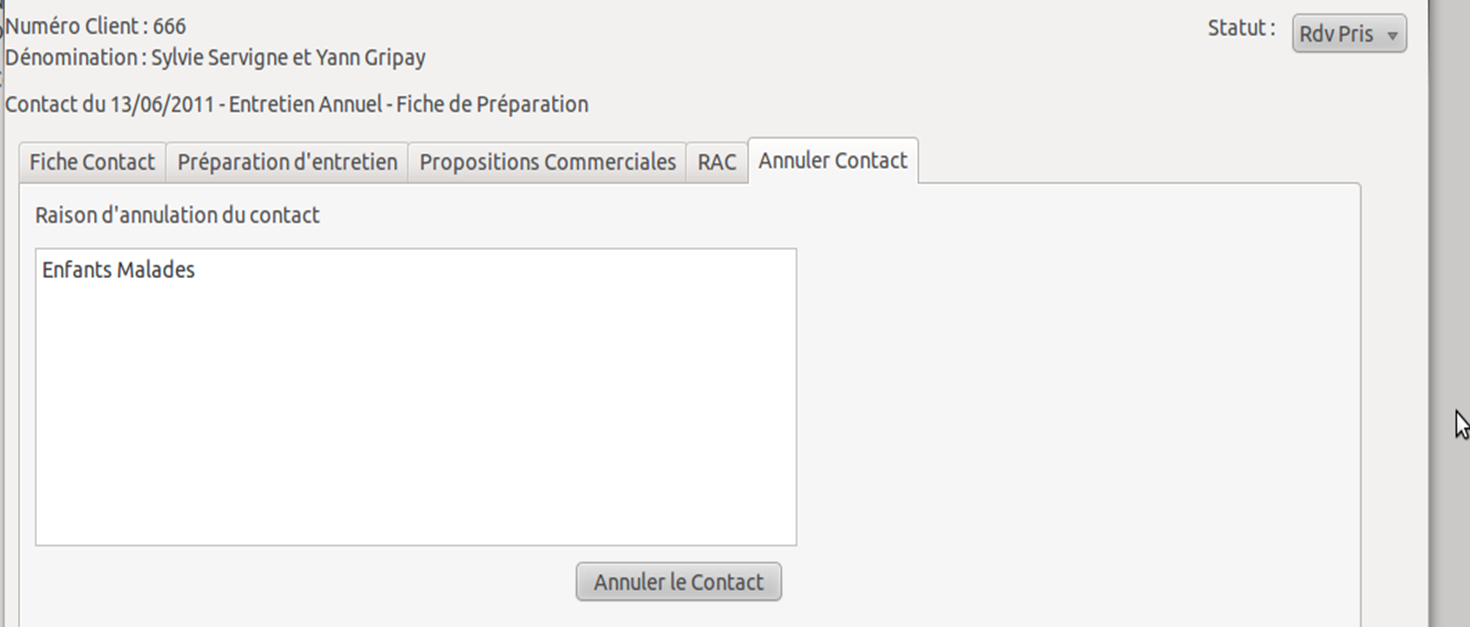
\includegraphics[width=10cm]{\PIXPATH/contact4}
\end{center}

\subsection{IHM Agence}

L'IHM Agence permet de consulter les agents dans une agence et des informations 
de base sur l'agence. S�lectionner un agent permet d'acc�der aux informations 
de l'agent, dont sa liste de client et son planning.

\begin{center}
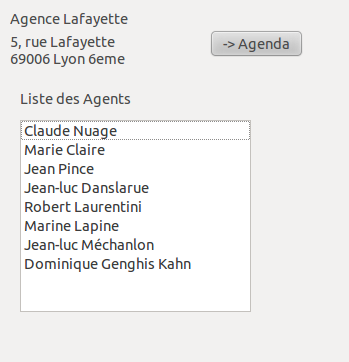
\includegraphics[width=10cm]{\PIXPATH/agence1}
\end{center}
\begin{center}
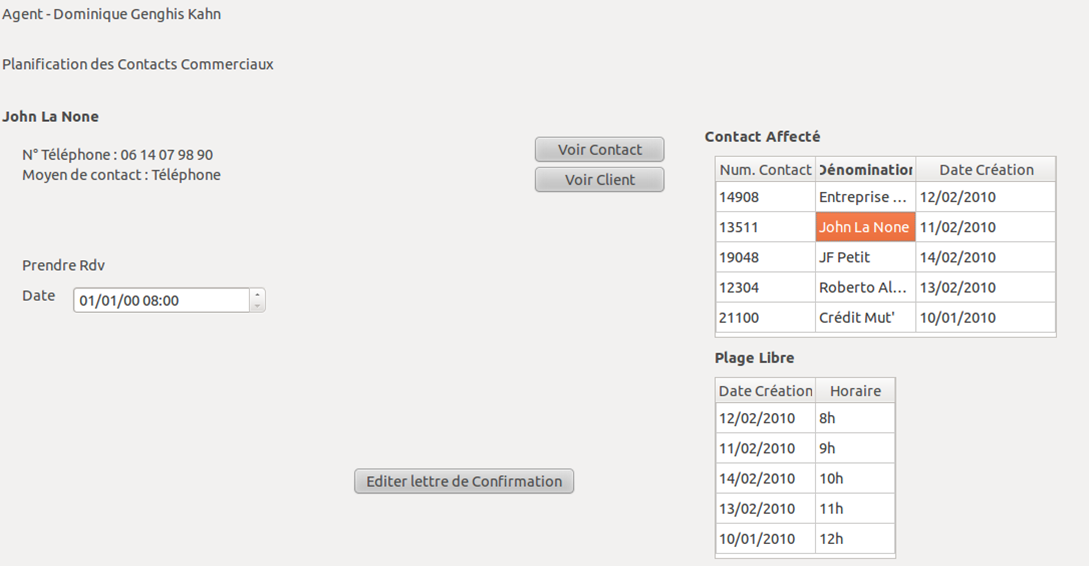
\includegraphics[width=10cm]{\PIXPATH/agence2}
\end{center}
\begin{center}
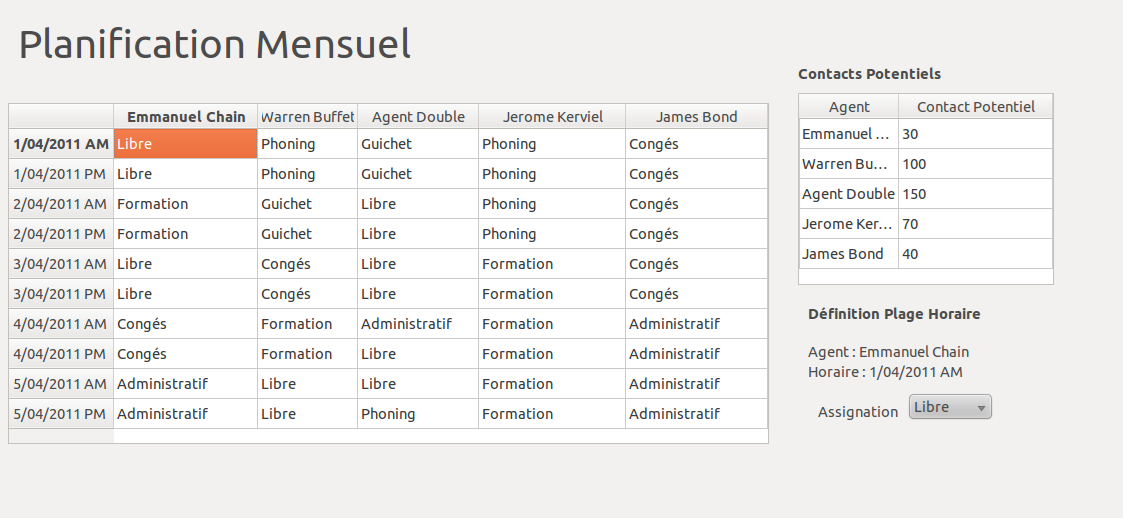
\includegraphics[width=10cm]{\PIXPATH/chef1}
\end{center}

\subsection{IHM �v�nement}
L'IHM �v�nements va permettre de consulter la liste des �v�nements arriv�s
durant la journ�e, de g�n�rer les motifs de contact correspondants puis les
contacts pr�vus.\\

� chaque �tape (�v�nements, motifs de contact et contacts pr�vus), la liste
des objets concern�s est visible et chaque objet peut �tre :
\begin{itemize}
\item Visualis� en d�tail
\item �dit�
\item Supprim�
\end{itemize}

\begin{center}
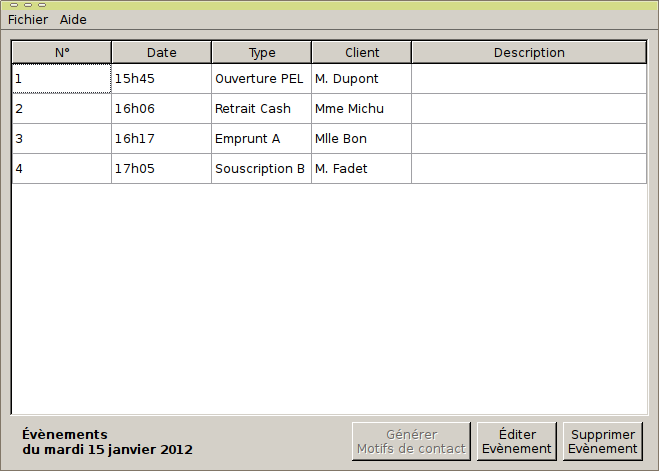
\includegraphics[width=10cm]{\PIXPATH/event1}
\end{center}
\begin{center}
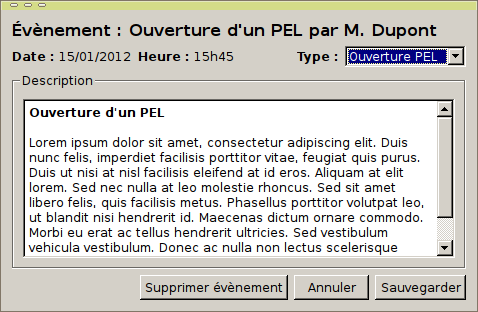
\includegraphics[width=10cm]{\PIXPATH/event2}
\end{center}